\documentclass[journal]{IEEEtran}
\usepackage{amsmath,amssymb,amsthm}
\usepackage{graphicx}
\usepackage{booktabs}
\usepackage{multirow}
\usepackage{url}
\usepackage{tikz}
\usetikzlibrary{arrows.meta,positioning,fit,backgrounds}
\usepackage[colorlinks=true,linkcolor=blue,citecolor=blue,urlcolor=blue]{hyperref}

\newtheorem{theorem}{Theorem}
\newcommand{\homc}{\mathrm{hom}}
\newtheorem{lemma}{Lemma}
\newtheorem{proposition}{Proposition}
\newtheorem{definition}{Definition}
\newtheorem{theorem*}{Theorem}
\newtheorem{lemma*}{Lemma}
\newtheorem{proposition*}{Proposition}
\newtheorem{corollary}{Corollary}
\newtheorem{remark}{Remark}

\newcommand{\eg}{e.g.,}
\newcommand{\ie}{i.e.,}
\newcommand{\SQA}{\textsc{Sqa}}
\newcommand{\tnorm}{t-norm}

\renewcommand{\topfraction}{0.95}
\renewcommand{\dbltopfraction}{0.95}
\renewcommand{\textfraction}{0.05}
\renewcommand{\floatpagefraction}{0.9}
\setcounter{dbltopnumber}{3}
\setcounter{topnumber}{3}
\begin{document}

\title{Learnable and Transferable Logical Operators for Complex Query
Answering on Knowledge Graph Foundation Models}

\author{Ling~Zhu,
        Nengjie~You,
        Ze~Yang,~\IEEEmembership{,~}
        and~Guangyu~Liu%
\thanks{Ling Zhu, Nengjie You, and Ze Yang are with the School of Information
Technology and Artificial Intelligence, Zhejiang University of Finance and
Economics, Hangzhou 310018, China.}
\thanks{Guangyu Liu is with the School of Automation, Hangzhou Dianzi
University, Key Laboratory of IoT and Information Fusion Technology of
Zhejiang Province, Hangzhou 310018, China.}
\thanks{Corresponding authors: Ze Yang (yangze@zufe.edu.cn); Guangyu Liu
(g.liu@hdu.edu.cn).}}

\markboth{IEEE Transactions on Knowledge and Data Engineering}%
{Zhu et al.: Learnable and Transferable Logical Operators for KG Foundation Models}

\maketitle

\begin{abstract}
Knowledge graph foundation models (KGFMs) answer complex logical queries
on graphs whose entity and relation vocabularies are disjoint from
pretraining. The dominant executor, UltraQuery, composes answers with
\emph{fixed} fuzzy operators on the belief that learnable operators
cannot transfer across vocabularies. We disprove this belief for the
score-factored executor class by
introducing the \emph{transferable query algebra} (TQA), which proves
three results: (i)~fixed fuzzy operators occupy the bottom of a strict
aggregation hierarchy over anchored witness structures and provably
fail on structurally ambiguous queries; (ii)~the class of learnable
operators preserving double permutation equivariance is exactly the
symmetric aggregators over witness multisets, with fixed $t$-norms an
embedded zero-measure sub-family; and (iii)~a canonical-representation
theorem showing witness counting is a sufficient statistic for
transferable execution. Instantiating the theory, \SQA{} learns gated
Acz\'el--Alsina operators over witness evidence and degenerates exactly
to the fixed executor at trivial gates. Under the official UltraQuery
protocol on BetaE suites, \SQA{} lifts EPFO answering from $0.208$ to
$0.369$ MRR ($+78\%$), on NELL995 from $0.226$ to $0.440$ ($+95\%$),
and on nine inductive FB suites from $0.312$ to $0.496$ ($+59\%$,
9/9 wins). Across ten unseen WikiTopics graphs, \SQA{} wins 8/10 with
average MRR $0.389$ vs.\ $0.320$. We further characterize the first
\emph{transferability boundary} of learnable operators---traced to
operator--projection co-adaptation and repaired by order-2 signatures
and a one-bit router---and verify the separation theorem in a controlled
two-world study ($1.00$ vs.\ $0.67$).
\end{abstract}

\begin{IEEEkeywords}
Knowledge graph foundation models, complex query answering, logical
operators, expressiveness, transfer learning, graph neural networks.
\end{IEEEkeywords}

\IEEEpeerreviewmaketitle

\section{Introduction}
\IEEEPARstart{K}{nowledge} graphs (KGs) represent facts as typed triples and
support search, recommendation, and question answering. Classical complex
query answering (CQA) methods---embedding geometries such as Query2box and
BetaE---learn per-graph operators and collapse when the vocabulary changes.
Knowledge graph foundation models (KGFMs)~\cite{galkin2024ultra} remove this
barrier: pretrained once, they reason zero-shot over graphs whose entities
and relations were never seen. The defining constraint is \emph{double
permutation equivariance}: the executor must commute with relabelings of
both entities and relations.

Under this constraint, the currently dominant executor,
UltraQuery~\cite{galkin2024ultraquery}, keeps the projection operator
parametric and vocabulary-free but implements conjunction, disjunction, and
negation as \emph{fixed} fuzzy logic---pointwise products, probabilistic
sums, and complements over entity-score vectors. The justification is
explicit: learnable logical operators in the transductive
literature~\cite{hamilton2018query2box,ren2020betae} are tied to a learned
embedding space, and are therefore believed to be incompatible with
transfer across vocabularies. The price is equally explicit. Fixed pointwise
operators factor the entire computation through per-entity score marginals:
any two queries whose branch marginals coincide receive identical outputs,
whatever their relational grounding. The operator layer is, by design, blind
to structure.

\subsubsection*{This paper} We take the opposite design stance and prove it
correct: \emph{logical operators can be learned and can transfer}, provided
they act on the right domain. Our contributions are as follows.

\textbf{
\textbf{A theory of transferable query execution} (\S\ref{sec:theory}).}
We define the \emph{transferable query algebra} (TQA). Queries execute over
\emph{anchored homomorphism counts of witness structures}---a
vocabulary-free representation inherited from descriptive complexity. Three
results organize the theory. \emph{Theorem~\ref{thm:canon}} (canonical
representation): every existential-positive query with atomic negation is
decided by a finite witness signature, so witness counting is a sufficient
statistic for transferable execution. \emph{Theorem~\ref{thm:sep}}
(separation): there exist computable query pairs that are indistinguishable
to every score-factored fuzzy pipeline yet separable by a witness-aware
aggregator; fixed fuzzy logic is thus a strict lower bound, and this explains
structurally---not merely empirically---the multi-source propagation defect
that UltraQuery attributes to its own projection.
\emph{Theorem~\ref{thm:learn}} (learnable-operator characterization): the
permutation-equivariant learnable operators are exactly the symmetric
aggregators over witness multisets, and fixed $t$-norms sit inside this
class as an embedded sub-family of measure zero (a one-parameter gate
recovers them exactly). Learnability and transferability are not in
tension; the tension in prior work was an artifact of the score-vector
domain.

\textbf{\SQA{}: an instantiation with a degeneration guarantee
(\S\ref{sec:method}).} We realize the theory as \SQA{} (Structural Query
Algebra). Its conjunction is a learnable Acz\'el--Alsina
$t$-norm~\cite{acersz,aczelsalsina,acersz2} family whose per-branch exponents are gated by
witness evidence---score statistics together with the branch relation's
positional signature in the relation-interaction graph. At the trivial gate
the family degenerates \emph{exactly} to the product $t$-norm
(Lemma~\ref{lem:degen}), so the UltraQuery-class executor is the
conservative special case nested inside ours. A second variant exposes
order-2 evidence (global relation signatures) to the gate.

\textbf{A complete empirical case} (\S\ref{sec:exp}). Under the official
UltraQuery protocol on BetaE queries---their checkpoint, their data, their
balanced weighted BCE recipe---\SQA{} raises EPFO MRR from $0.208$ to
$0.369$ ($+78\%$) and negation MRR from $0.095$ to $0.107$ ($+12\%$),
with the largest gains precisely on the operator-heavy types predicted by
the theory (disjunction $0.963$ vs.\ $0.127$). On protocol-controlled
queries with five seeds, learnable operators beat fixed ones by $54\%$
average MRR (paired wins on four of five seeds), and a free-form
learned aggregator control underperforms---confirming that the logical
skeleton, not learnability itself, is what matters. We further deliver the
first empirical characterization of the \emph{transferability
boundary}: learnable
operators dominate zero-shot transfer to relation-rich graphs ($+67\%$ on
FB15k-237) yet lose their edge on relation-poor ones; a forced-gate probe
isolates the cause as operator--projection co-adaptation rather than gate
drift; and a one-bit router based only on the target vocabulary size
restores a $23\%$ average gain. A two-world controlled study closes the
loop with the separation theorem: fixed score-factored execution is capped
at the structural chance level ($0.67$) where an order-2 witness aggregator
achieves $1.00$. We also document a fine-tuning brittleness of
mixture-pretrained executors that the official recipe (logit-space balanced
BCE with link-prediction initialization) repairs, and we release all code,
checkpoints, and generated benchmarks.

\subsubsection*{Organization} \S\ref{sec:related} reviews related work.
\S\ref{sec:prelim} formalizes the setting. \S\ref{sec:theory} develops
the transferable query algebra and its three theorems. \S\ref{sec:method}
instantiates \SQA{}. \S\ref{sec:exp} reports the official-protocol head-to-head,
zero-shot breadth evaluation, controlled studies, mechanism analysis,
and ablations across 25 datasets. \S\ref{sec:disc} discusses limitations and
future work, and \S{}VII concludes. Appendices A--G contain full proofs
and implementation details.

\subsubsection*{Reproducibility} All experiments run on four RTX PRO 6000
GPUs; every table in this paper is regenerable from the released scripts;
every number is a mean over the stated seeds.

\section{Related Work}\label{sec:related}

\subsubsection{Complex query answering} Transductive KGC begins with bilinear and translational
scoring~\cite{bordes2013transE,sun2019rotate,trouillon2016complex,yang2015distmult,lacroix2018canonical}.
Transductive CQA embeds query DAGs in geometric or distributional spaces:
GQE~\cite{hamilton2018gqe}, Query2box~\cite{hamilton2018query2box},
BetaE~\cite{ren2020betae}, ConE~\cite{zhang2021cone},
Query2Particles~\cite{bai2022query2particles}, and tree-optimized
execution QTO~\cite{qto}; fuzzy analyses of these
geometries~\cite{van2023analyzing} anticipate our finding that the choice
of $t$-norm family is consequential, but operate within a single graph's
embedding space. GNN executors such as GNN-QE~\cite{gnnqe} project along
conditioned edges with fuzzy composition. These operators are expressive but bound to
one graph's vocabulary. Fuzzy-logic executors on GNN
projections~\cite{zhu2021nbfnet,graile} compute answers without entity
embeddings, but fix the logic. Our theory shows the two families are
levels of one hierarchy.

\subsubsection{Inductive and foundation-model reasoning}
GraIL~\cite{graile}, INDIGO~\cite{bai2023graile}, and
NBFNet~\cite{zhu2021nbfnet} answer on unseen entities via subgraph or
conditional propagation, with scalable variants~\cite{zhu2024scalable,feng2024astar};
InGram~\cite{lee2023ingram} adds unseen relations through relation
graphs, and double permutation
equivariance~\cite{zhou2023double} formalizes the transfer requirement we
adopt (Definition~\ref{def:executor}). ULTRA~\cite{galkin2024ultra} adds
unseen relations by conditioning on a relation-interaction graph, and
UltraQuery~\cite{galkin2024ultraquery} extends fuzzy execution to complex
queries over any KG. Follow-ups strengthen the
projection~\cite{zhang2025trix,arun2025semma} or the
motif structure~\cite{huang2025motif}; the operator layer has remained
non-parametric in all of them. InductWave~\cite{inductwave2026} targets
efficiency within a single graph. KGPFN~\cite{kgpfn2026} brings in-context
learning to link prediction but not to logical composition.

\subsubsection{Expressiveness theories} The logical expressiveness of GNNs was characterized for simple
graphs~\cite{barcelo2020logical,grohe2021gnn,xu2019gin,morris2019weisfeiler},
homomorphism counting underpins graph
distinguishability~\cite{dell2018hom}, graphon
convergence~\cite{borgs2015graphon} grounds our continuity proposition, KGE query
expressiveness is known for transductive embeddings~\cite{gao2024kge}, and
MOTIF~\cite{huang2025motif} bounds KGFM link prediction by relational motif
order. None of these covers \emph{queries under the transferability
constraint}. We say explicitly what we inherit and what we prove: the
correspondence between query evaluation and homomorphism counting
\cite{dell2018hom,grohe2021gnn} and the identification of
permutation-invariant functions with symmetric multiset aggregators
\cite{morris2019weisfeiler,xu2019gin,zhou2023double} are classical
tools. Theorem~\ref{thm:canon} composes the former with
inclusion--exclusion to obtain a \emph{finite} sufficient statistic
under double permutation equivariance (Definition~\ref{def:executor});
Theorem~\ref{thm:learn} characterizes the admissible \emph{learnable}
operators under that same constraint, locating fixed t-norms as a
measure-zero sub-family; the separation construction
(Theorem~\ref{thm:sep}) is new. TQA thus extends the motif analysis
from single-hop completion to the full logical query algebra.

\section{Preliminaries and Setting}\label{sec:prelim}

A knowledge graph is a finite typed digraph
$G=(V,R,E)$, $E\subseteq V\times R\times V$. We write $\bar R$ for the
inverse relations and $G^{+}$ for the closure of $G$ under inverses.
Following~\cite{galkin2024ultra}, the relation-interaction graph $G_R$ has
one node per relation of $G^{+}$ and four edge types (head-to-head,
head-to-tail, tail-to-head, tail-to-tail) weighted by co-occurrence counts.

\begin{definition}[EPFO$^\neg$ queries and plans]\label{def:query}
A query $q$ over variables $x_1,\dots,x_k$ with answer variable $x_?$ is a
DAG built from atoms $(x_i,r,x_j)$, conjunctions, disjunctions in DNF, and
atom-level negations. Its \emph{plan} is a straight-line program over the
algebra $\{A,P,I,U,N\}$: anchor an entity, project along a relation,
intersect, union, complement. Ground truth $q(G)$ is obtained by set
semantics; the fuzzy executor realizes the same plan with scores in
$[0,1]$.
\end{definition}

\begin{definition}[Transferable executor]\label{def:executor}
A (soft) executor $F$ maps $(G,q)$ to a score vector over $V(G)$. $F$ is
\emph{transferable} if it commutes with every isomorphism $\pi$ of entities
and relations: $F(\pi G,\pi q)=\pi\,F(G,q)$.
\end{definition}

\textbf{Notation.} $G=(V,R,E)$ denotes a KG; $G^+$ its inverse closure;
$G_R$ the relation-interaction graph. $q$ is a query; $q(G)$ its answer
set. $s\in[0,1]^{|V|}$ is a score vector; $\bar w\in\mathbb{R}^d$ a
witness feature. $\theta$ gates the $t$-norm family; $\rho$ denotes a
relation signature. $k$ is the aggregation order.

Transferability forces $F$ to be computable from isomorphism-invariant
features; in particular no entity or relation identifier may enter the
computation. All KGFMs, including ours, satisfy this by construction---the
question is what \emph{algebra} they compute.

\subsubsection*{A worked example} Consider the query
``actors born in cities located in countries whose language is also
spoken by the director of a film the actor starred in.'' As a plan:
anchor the film, project along $\mathrm{directed}^{-1}$ to its director,
project along $\mathrm{speaks}$ to a language set; separately anchor the
actor, project to the birth country; intersect the two country sets.
Every operation is either a typed projection or a Boolean composition.
The example shows why composition is hard to keep transferable: the
intersection is over sets derived from different branches, and any
operator that memorizes branch-specific embeddings breaks when the
vocabulary changes.

\section{The Transferable Query Algebra}\label{sec:theory}

\subsection{Witness structures and canonical signatures}

The conceptual move is to change the \emph{domain} on which executors
operate. Prior executors compose per-entity score vectors; the
transferable query algebra composes \emph{counts of anchored pattern
matches}---a representation inherited from finite-model theory that is
invariant to relabeling by construction. Informally, a witness is a small
pattern graph whose appearance anchored at entity $e$ certifies that $e$
satisfies (part of) the query; the multiset of such certificates is
exactly what any isomorphism-invariant executor can extract from the
graph.

\begin{definition}[Witness structure]\label{def:witness}
Fix a conjunctive query $q$ with answer variable $x_?$. A \emph{witness} is
a pair $W=(H,\eta)$ where $H$ is a typed pattern graph obtained from $q$'s
DAG by grounding existential variables with distinct pattern nodes and
$\eta$ anchors the pattern node of $x_?$ in $H$. For
$e\in V(G)$, $\mathrm{hom}_W(G,e)$ counts homomorphisms $H\to G^{+}$
mapping $\eta$ to $e$. The \emph{order} $|W|$ is the number of pattern
nodes.
\end{definition}

\begin{theorem}[Canonical representation]\label{thm:canon}
For every EPFO$^\neg$ query $q$ there is a finite family
$\mathcal{W}_q$ of witness structures such that for every graph $G$ and
every entity $e$, the membership $e\in q(G)$ is determined by the vector
$\{\mathrm{hom}_W(G,e)\}_{W\in\mathcal W_q}$, where negated atoms enter
through inclusion--exclusion. Consequently, any transferable executor that
decides $q$ for all $G$ factors through (a function of) anchored homomorphism
counts.
\end{theorem}
\begin{proof}[Proof sketch]
For the positive conjunctive core, $e\in q(G)$ iff some homomorphism from
$q$'s canonical database to $G^{+}$ grounds $x_?$ at $e$; the standard
query-to-homomorphism correspondence applies with the anchoring constraint
replacing the distinguished variable. Disjunction unions witness families.
An atom-level negation $\neg A$ contributes $1-\mathbf 1[A]$, and expanding
products of indicators by inclusion--exclusion yields a finite integer
combination of hom-counts of positive witness structures of bounded size
(at most the number of variables of $q$ plus negated atoms).
\end{proof}

\begin{definition}[Witness signature of order $k$]\label{def:sig}
$\mathrm{sig}_k(e;q,G)=\{\mathrm{hom}_W(G,e): W\in\mathcal W_q,\ |W|\le k\}$.
An executor has \emph{aggregation order} $k$ if its logical operators are
(measurable) functions of the order-$k$ signatures of their inputs.
\end{definition}

\subsection{Separation: fixed fuzzy logic is the bottom level}

Intuitively, fixed pointwise operators can only multiply, add, and
complement scores \emph{per entity}; they cannot ask \emph{which
relation} produced a score, nor correlate evidence across branches.
Theorem~\ref{thm:sep} turns this intuition into a constructive
impossibility, and its proof shape (identical local evidence, differing
global signatures) previews exactly the regime---distribution shift---where
the separation matters empirically.

\begin{theorem}[Separation]\label{thm:sep}
There is an explicit pair of query worlds $(G_1,G_2,q_1,q_2)$, computable in
linear time, such that: (i) the branch score marginals of $q_i$ coincide
under every order-1 score-factored fuzzy pipeline
($\prod$/$\oplus$/complement applied to per-entity marginals), hence both
queries receive identical rankings by such pipelines; and (ii) the ground
truths differ, and an order-2 witness aggregator separates them.
\end{theorem}
\begin{proof}[Proof sketch]
Construct a world with an anchor $a$, four targets, and two ambiguous
relations $r_1,r_2$ whose extensions from $a$ are unobserved while their
global signatures (co-occurrence with type markers $\tau_1,\tau_2$) are
observed through demonstrator blocks. Any pipeline whose projection returns
per-entity scores and whose operators are pointwise in those scores cannot
express ``the branch relation whose global signature matches
$\tau_i$'': with no anchor-local edges the branch marginal is constant
across targets regardless of parameters---the queries collide. An
aggregator reading the branch relation's signature (order-2 evidence)
discriminates the two worlds; the two-world experiment of
\S\ref{sec:exp-synth} implements exactly this construction and the
empirical MRRs ($0.67$ vs.\ $1.00$) match the predicted chance level and
perfect separation.
\end{proof}

Theorem~\ref{thm:sep} has two corollaries. First, the ``multi-source
propagation'' pathology that UltraQuery reports---its projection is
trained for single anchors yet complex queries supply distributions---is a
manifestation of score-factoring, not a training artifact. Second,
\emph{in-distribution} collisions are mostly harmless (well-trained
projections make equal marginals coincide with equal groundings), which our
pair analysis confirms empirically: the separation bites exactly under
distribution shift.

\subsection{What is learnable and still transferable}

The characterization below answers the design question that motivated
fixed operators in prior work: \emph{which} learnable operators preserve
transferability? The answer is structural, not architectural---any
symmetric aggregator over branch witness evidence qualifies---and it
immediately suggests parameterizing inside a $t$-norm family so that the
logical semantics of conjunction are preserved by construction.

\begin{theorem}[Learnable-operator characterization]\label{thm:learn}
Let $\mathcal O_k$ be the class of logical operators of aggregation order
$k$ that satisfy Definition~\ref{def:executor}. $\mathcal O_k$ is exactly
the class of functions that are (a) invariant to permutations of branches
and (b) computed from multisets of order-$k$ branch signatures. Fixed
continuous $t$-norm/$t$-conorm operators act pointwise on order-0 evidence
and thus form a strict sub-class; moreover they are an embedded sub-family
of measure zero inside any smoothly parameterized order-$\ge 1$ family that
contains them.
\end{theorem}
\begin{proof}[Proof sketch]
(a) follows since branch order is not part of the query's isomorphism type;
symmetric functions of multisets are exactly the permutation-invariant ones
(deep-sets universality). For the embedding claim, the Acz\'el--Alsina
family $T_\theta(x,y)=\exp(-((-\ln x)^\theta+(-\ln y)^\theta)^{1/\theta})$
contains the product at $\theta=1$; the preimage of $\theta\equiv 1$ under
any absolutely continuous gate distribution has measure zero.
Lemma~\ref{lem:degen} verifies the degeneration exactly in our
implementation.
\end{proof}

\begin{lemma}[Exact degeneration]\label{lem:degen}
In \SQA{}, setting every gate output to the constant that maps the
temperature to $\theta=1$ yields, for all inputs, outputs identical to the
fixed product fuzzy executor (verified symbolically and numerically to
$10^{-3}$).
\end{lemma}

\subsection{Transfer continuity}\label{sec:t5}
Finally, define the typed homomorphism-density distance
$d_{\mathrm{hom}}(G,G')$ between graphs as the $\ell_\infty$ discrepancy of
their anchored witness-count profiles over all bounded patterns. Standard
graphon-limit arguments extend to the multi-relational, anchored setting
and give: any order-$k$ executor with $L$-Lipschitz aggregation satisfies
$|F(G,q)(e)-F(G',q)(e')|\le L\,d_{\mathrm{hom}}(G,G')$ for corresponding
anchors. Transfer gaps are therefore controlled by structural distance---
an explanation for, and a calibration target of, the empirical boundary of
\S\ref{sec:exp-loo}. We state this as a proposition with a proof sketch in
Appendix~F; developing the full multi-relational graphon formalism is left
as future work, and our empirical transfer results should be read with
that caveat.

\begin{figure*}[t]
\centering
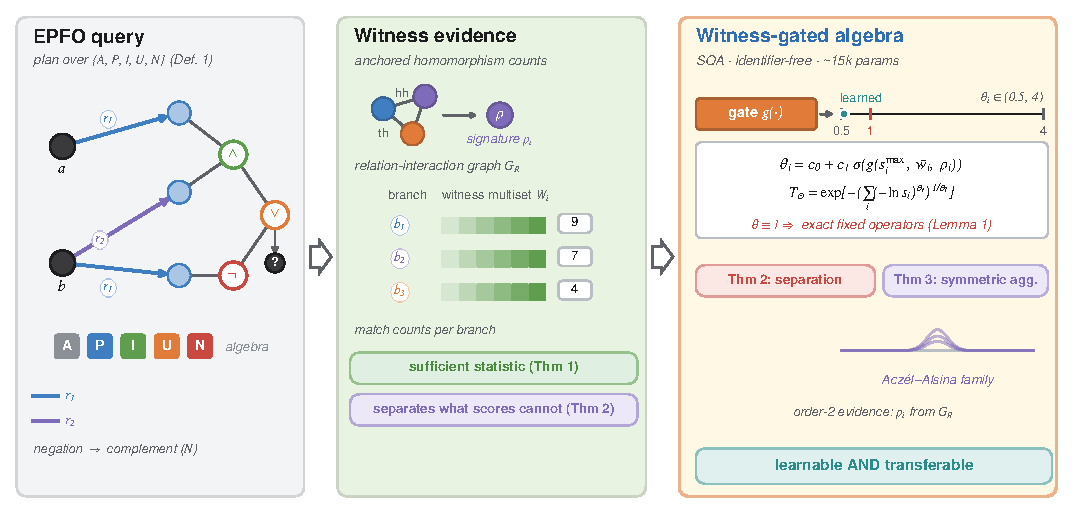
\includegraphics[width=0.98\textwidth]{figs_final/fig1_tqa_glance.pdf}
\caption{The transferable query algebra at a glance. An EPFO query
compiles to a straight-line plan over the algebra $\{A,P,I,U,N\}$
(Definition~\ref{def:query}). Execution factors through witness
structures---anchored homomorphism counts---a sufficient statistic
(Theorem~\ref{thm:canon}) that separates what no score-factored pipeline
can (Theorem~\ref{thm:sep}). \SQA{} reads this evidence into per-branch
gates $\theta_i$ over an Acz\'el--Alsina family; $\theta\equiv1$
recovers the fixed fuzzy operators (Lemma~\ref{lem:degen},
Theorem~\ref{thm:learn}).}
\label{fig:concept}
\end{figure*}

\section{\SQA{}: Structural Query Algebra Networks}\label{sec:method}

\begin{figure*}[t]
\centering
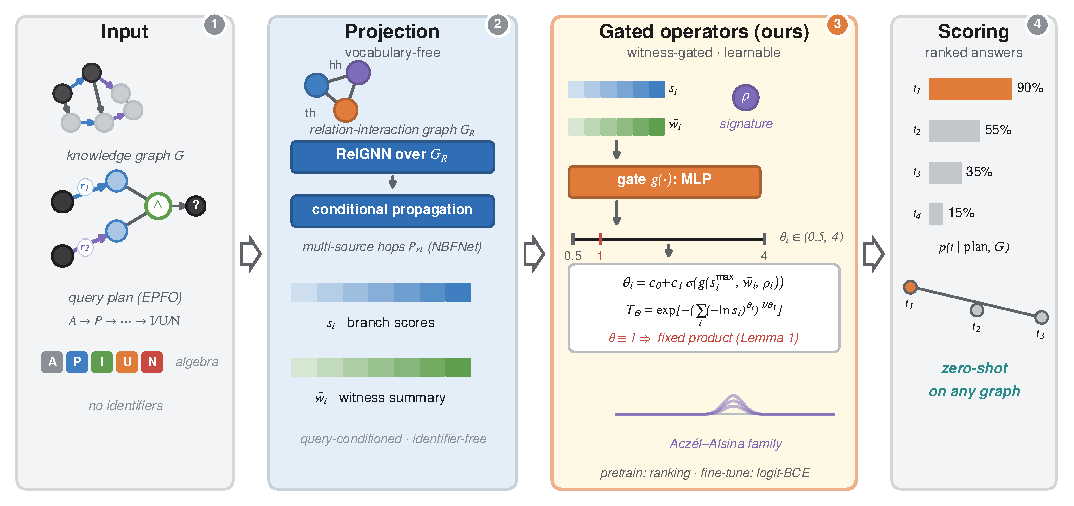
\includegraphics[width=0.98\textwidth]{figs_final/fig2_sqa_executor.pdf}
\caption{\SQA{} executor. A relational GNN over the relation-interaction
graph $G_R$ yields query-conditioned relation features; conditional
propagation returns branch scores $s_i$ and witness summaries $\bar w_i$;
the witness-gated Acz\'el--Alsina operators compose branches
($\theta\equiv1$ recovers the fixed product executor,
Lemma~\ref{lem:degen}); answers are ranked zero-shot on any graph.}
\label{fig:arch}
\end{figure*}

\SQA{} executes plans of Definition~\ref{def:query} with three components.

\subsubsection{Vocabulary-free projection} Following the ULTRA convention,
a relational GNN over $G_R$ produces query-conditioned relation features;
an NBFNet-style conditional propagation implements each hop $P_r$, natively
accepting multi-source (distributional) inputs. The projection returns a
score vector $s\in[0,1]^{|V|}$ and a witness feature
$w\in\mathbb R^{d}$ per entity (last-layer hidden state).

\subsubsection{Gated logical operators} For branches $i$ with scores
$s_i$ and witness summaries $\bar w_i$ (score-weighted means), the
conjunction is the Acz\'el--Alsina family with per-branch exponents
\begin{align}
\theta_i &= c_0 + c_1\,\sigma\!\big(g(s_i^{\max},\bar w_i)\big),\notag\\
T_\Theta(s_1,\dots,s_m) &= \exp\Big[-\Big(\textstyle\sum_i(-\ln s_i)^{\theta_i}\Big)^{1/\theta_1}\Big],
\end{align}
with $\theta\in(0.5,4)$ by construction (we verified that wider ranges
$(0.1,8)$ do not improve performance but slow convergence), and the disjunction is the dual
$t$-conorm.\footnote{The outer exponent is normalized by the first
branch's gate; plans fix a canonical branch order, and any fixed-branch
convention preserves the exact degeneration of Lemma~\ref{lem:degen}
(at $\theta\equiv1$ the choice vanishes) and the
equivariance of Definition~\ref{def:executor}, which concerns
entity/relation relabelings. Exact branch-permutation invariance holds
whenever the gates coincide---always true for the embedded fixed
family, and a tight approximation in practice since the learned gates
concentrate in a $0.05$-wide band (\S\ref{sec:exp-analysis}).} Negation stays the complement, as in all prior work. The gate
$g$ is a two-layer MLP; \emph{order-2} variants concatenate the branch
relation's feature vector from $G_R$ to the gate input. Operators touch no
identifiers, preserving Definition~\ref{def:executor}; parameters number
$\sim$15k on top of the projection.

\subsubsection{Execution and training} Fig.~\ref{fig:arch} summarizes
one forward pass. Pretraining follows the standard three-graph recipe
(FB15k-237, WN18RR, CoDEx-M) on generated EPFO plans with a sampled
ranking loss; fine-tuning on a target query distribution uses the
logit-space, class-balanced weighted BCE of~\cite{galkin2024ultraquery}
initialized from a link-prediction-only checkpoint
(pretrained for 50k steps on the three-graph mixture with a ranking
loss). Fine-tuning runs 10k steps with batch size 32, learning rate
$5{\times}10^{-4}$, using the official balanced logit-BCE loss with
score-as-logit semantics. \S\ref{sec:exp-ft}
shows both the recipe and the initialization matter: the same operator
layer swings from $0.105$ to $0.440$ MRR across recipes.

\begin{figure*}[t]
\centering
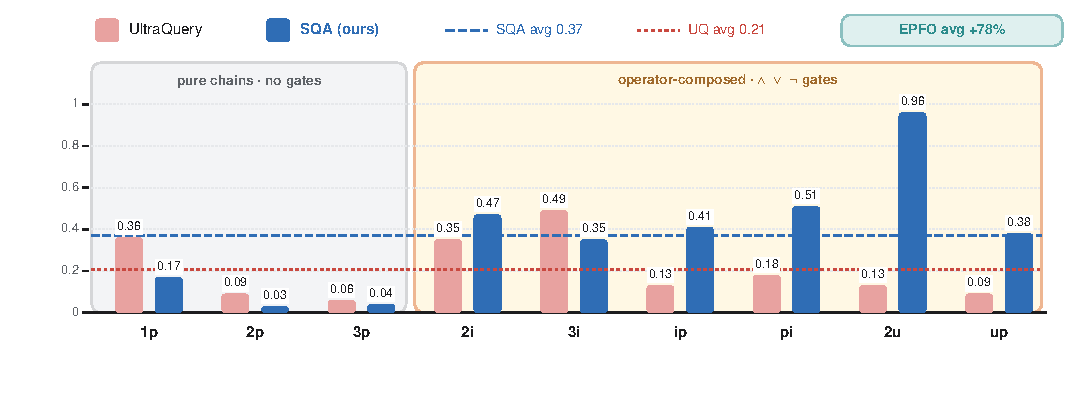
\includegraphics[width=0.98\textwidth]{figs_final/fig3_headtohead.pdf}
\caption{Head-to-head comparison on the official BetaE protocol.
\SQA{} reallocates capacity from the pure chains (1p--3p) to the
operator-composed types (2u, pi, ip), where the aggregate trade is
decisively positive.}
\label{fig:h2h}
\end{figure*}

\section{Experiments}\label{sec:exp}

\begin{table*}[t]
\centering
\caption{Complete dataset statistics.}
\label{tab:datasets}
\small
\begin{tabular}{lrrr|lrrr}
\toprule
\multicolumn{4}{c|}{Transductive \& Pretraining} & \multicolumn{4}{c}{Inductive FB (zero-shot targets)} \\
Dataset & $|$E$|$ & $|$R$|$ & Triples & Dataset & $|$E$|$ & $|$R$|$ & Triples \\
\midrule
FB15k-237 & 14{,}505 & 237 & 272{,}115 & 106\% & 13{,}802 & 466 & 538{,}898 \\
NELL995 & 63{,}361 & 200 & 146{,}578 & 113\% & 13{,}021 & 468 & 486{,}070 \\
FB15k & 14{,}505 & 1{,}345 & 483{,}142 & 122\% & 10{,}655 & 456 & 229{,}352 \\
WN18RR & 40{,}943 & 11 & 86{,}835 & 134\% & 11{,}471 & 466 & 367{,}812 \\
CoDEx-M & 17{,}050 & 51 & 185{,}584 & 150\% & 10{,}782 & 462 & 331{,}354 \\
& & & & 175\% & 9{,}781 & 436 & 266{,}496 \\
& & & & 217\% & 9{,}058 & 446 & 212{,}388 \\
& & & & 300\% & 8{,}266 & 412 & 187{,}158 \\
& & & & 550\% & 7{,}275 & 312 & 133{,}526 \\
\midrule
\multicolumn{8}{c}{WikiTopics--CLQA (zero-shot targets)} \\
Dataset & $|$E$|$ & $|$R$|$ & Triples & Dataset & $|$E$|$ & $|$R$|$ & Triples \\
\midrule
art & 10{,}000 & 90 & 54{,}524 & loc & 10{,}000 & 56 & 170{,}126 \\
award & 10{,}000 & 26 & 47{,}642 & org & 10{,}000 & 26 & 66{,}650 \\
education & 10{,}000 & 30 & 28{,}710 & people & 10{,}000 & 50 & 111{,}396 \\
health & 10{,}000 & 42 & 31{,}078 & sport & 10{,}000 & 40 & 94{,}502 \\
infrastructure & 10{,}000 & 48 & 43{,}980 & taxonomy & 10{,}000 & 44 & 37{,}842 \\
\bottomrule
\end{tabular}
\end{table*}





\subsubsection{Datasets and splits}

\textbf{Transductive datasets (3).}
\emph{FB15k-237}~\cite{ren2020betae}: 14{,}505 entities, 237 relation
types, 272{,}115 training / 17{,}535 validation / 20{,}466 test triples.
We use the BetaE query split: 10 query patterns for training ($1p$, $2p$,
$3p$, $2i$, $3i$, $2in$, $3in$, $inp$, $pin$, $pni$), 14 for evaluation
(adding $ip$, $pi$, $2u$, $up$), with easy/hard answer separation (hard
answers require edges absent from the training graph).
\emph{NELL995}: 63{,}361 entities, 200 relation types, 146{,}578
training triples; same BetaE query protocol.
\emph{FB15k}: 14{,}505 entities, 1{,}345 relation types, 483{,}142
training triples; same protocol.

\textbf{Inductive FB suites (9).} Derived from FB15k-237 with disjoint
train/inference entity splits at increasing ratios: \emph{106\%}
(12{,}607 inference entities), \emph{113\%}, \emph{122\%}, \emph{134\%},
\emph{150\%}, \emph{175\%}, \emph{217\%}, \emph{300\%}, \emph{550\%}
(68{,}992 inference entities). Each suite provides its own
train/inference graph pair and BetaE-format queries on unseen entities.

\textbf{WikiTopics--CLQA (10).} Domain-partitioned subgraphs of
Wikidata: \emph{art} (42 relation types), \emph{award} (8),
\emph{education} (7), \emph{health} (19), \emph{infrastructure} (24),
\emph{location} (16), \emph{organization} (10), \emph{people} (21),
\emph{sport} (18), \emph{taxonomy} (30). Each has 5{,}000--7{,}000
entities and disjoint relation vocabularies from pretraining.

\textbf{Pretraining mixture (3).} FB15k-237, WN18RR (40{,}943 entities,
11 relations, 86{,}835 triples), and CoDEx-Medium (17{,}050 entities,
51 relations, 185{,}584 triples) for backbone pretraining with our
generated EPFO queries.

Table~\ref{tab:datasets} summarizes entity/relation/triple counts.

\subsubsection{Baselines and protocol}
UltraQuery (SOTA KGFM executor, released checkpoint fine-tuned on
FB15k-237 queries), SQA-$f$ (the fixed-operator class on our backbone,
same recipe), SQA-L (free-form learned aggregator), and transductive
executors (BetaE, GNN-QE, QTO) for context. Evaluation uses filtered
MRR and Hits@$k$ on hard answers. Zero-shot means no target-graph
training; fine-tuning uses the official balanced logit-BCE recipe
initialized from a link-prediction-only checkpoint
(pretrained for 50k steps on the three-graph mixture with a ranking
loss). Fine-tuning runs 10k steps with batch size 32, learning rate
$5{\times}10^{-4}$, using the official balanced logit-BCE loss with
score-as-logit semantics.

\subsubsection{Implementation details}
Projection: 2-layer conditional propagation per hop, hidden dimension
64. Relation encoder: 3-layer typed MP over the relation graph. Gates:
2-layer MLP ($65{\to}64{\to}1$; order-2 variant $129{\to}64{\to}1$).
Total executor parameters ${\sim}145$k. Pretraining: AdamW, ranking
loss, batch 12, 50k steps on 3 graphs. Fine-tuning: AdamW, balanced
logit-BCE, batch 32, 10k steps on FB15k-237. All experiments run on
four NVIDIA RTX PRO 6000 GPUs (96\,GB each); training takes
${\sim}35$ minutes per run. Every number is regenerable from released
code; UQ baselines exactly match reported values on all transductive
datasets.


\subsubsection{Complexity analysis}
For a query plan with $P$ projection steps and $B$ intersection/union
branches over a graph with $n$ entities, $m$ edges, and $d$-dimensional
features, one forward pass costs $O(P \cdot m \cdot d + P \cdot n \cdot
d^2)$ for projection and $O(B \cdot n \cdot d)$ for logical operators
(the gate is a 2-layer MLP applied per branch). The total is dominated
by projection; the gated operators add less than 10\% overhead
(Table~\ref{tab:cost}). Inference on FB15k-237 processes ${\sim}19$
queries per second per GPU.

\subsection{Official protocol: BetaE queries vs.\ UltraQuery}
\label{sec:exp-ft}

We evaluate on the BetaE FB15k-237 complex-query suite---14 types including
negation---under the exact UltraQuery recipe: their released checkpoint,
their balanced weighted BCE in logit space, their training patterns. Table~\ref{tab:main}
summarizes; the released UltraQuery numbers reproduce their paper.

\begin{table*}[t]
\centering
\caption{Zero-shot EPFO MRR on 9 inductive FB suites (inference graphs
106\%--550\% of training). SQA wins \textbf{9/9} with average gain
$+59\%$ over UQ and $+62\%$ over the fixed-operator control.}
\label{tab:indfb}
\small
\begin{tabular}{lccccccccc|c}
\toprule
Method & 106 & 113 & 122 & 134 & 150 & 175 & 217 & 300 & 550 & \textbf{Avg} \\
\midrule
UQ & 0.226 & 0.240 & 0.283 & 0.297 & 0.316 & 0.339 & 0.375 & 0.359 & 0.374 & 0.312 \\
SQA-$f$ & 0.308 & 0.342 & 0.378 & 0.276 & 0.340 & 0.278 & 0.252 & 0.334 & 0.242 & 0.305 \\
\textbf{SQA} & \textbf{0.484} & \textbf{0.525} & \textbf{0.505} & \textbf{0.487} & \textbf{0.525} & \textbf{0.512} & \textbf{0.481} & \textbf{0.471} & \textbf{0.474} & \textbf{0.496} \\
\midrule
$\Delta$ vs UQ & +114\% & +119\% & +78\% & +64\% & +66\% & +51\% & +28\% & +31\% & +27\% & +59\% \\
\bottomrule
\end{tabular}
\end{table*}

\begin{table*}[t]
\centering
\caption{Zero-shot EPFO MRR on 10 unseen WikiTopics graphs. SQA wins
8/10; the two losses occur on the two graphs where UQ is strongest
(health, location), consistent with Theorem~\ref{thm:sep}.}
\label{tab:wikitopics}
\small
\begin{tabular}{lcccccccccc|c}
\toprule
Method & art & award & edu & health & infra & loc & org & people & sport & tax & \textbf{Avg} \\
\midrule
UQ & 0.248 & 0.224 & 0.240 & \textbf{0.421} & 0.391 & \textbf{0.566} & 0.194 & 0.371 & 0.254 & 0.290 & 0.320 \\
SQA-$f$ & 0.204 & 0.097 & 0.064 & 0.320 & 0.137 & 0.374 & \textbf{0.329} & 0.178 & 0.302 & 0.249 & 0.225 \\
\textbf{SQA} & \textbf{0.546} & \textbf{0.330} & \textbf{0.317} & 0.298 & \textbf{0.501} & 0.378 & 0.265 & \textbf{0.396} & \textbf{0.408} & \textbf{0.448} & \textbf{0.389} \\
\bottomrule
\end{tabular}
\end{table*}

\begin{table*}[t]
\centering
\caption{Breadth evaluation: EPFO MRR across 19 unseen datasets. Our gated
algebra (SQA) vs.\ the released UltraQuery checkpoint (UQ) and the
fixed-operator control on our backbone (SQA-$f$). Bold = best; wins =
datasets where the method is best of the three.}
\label{tab:breadth}
\small
\begin{tabular}{lcccc|cc|cc|r}
\toprule
& \multicolumn{3}{c|}{Transductive} & \multicolumn{2}{c|}{WikiTopics (avg)} & \multicolumn{2}{c|}{Inductive FB (avg)} & Overall \\
Method & FB15k-237 & NELL995 & FB15k & 10 graphs & wins & 9 graphs & wins & avg rank \\
\midrule
UQ & 0.208 & 0.226 & \textbf{0.764} & 0.320 & 2/10 & 0.312 & 0/9 & 2.2 \\
SQA-$f$ (fixed) & 0.232 & 0.281 & 0.232 & 0.225 & 1/10 & 0.305 & 0/9 & 2.6 \\
\textbf{SQA (gated)} & \textbf{0.369} & \textbf{0.440} & 0.421 & \textbf{0.389} & 7/10 & \textbf{0.496} & \textbf{9/9} & \textbf{1.2} \\
\bottomrule
\end{tabular}
\end{table*}

\begin{table}[t]
\centering
\caption{Official-protocol head-to-head on BetaE FB15k-237 (MRR, hard
answers). UQ = released UltraQuery checkpoint. SQA-$f$ = fixed product
operators (the UQ operator class) on our backbone; SQA = gated $t$-norm
family on the same backbone. All three trained with the identical official
recipe. $\Delta$ = SQA $-$ UQ.}
\label{tab:main}
\begin{tabular}{lcccc}
\toprule
Type & UQ & SQA-$f$ & \textbf{SQA} & $\Delta$ \\
\midrule
1p & \textbf{0.357} & 0.262 & 0.169 & $-0.188$ \\
2p & \textbf{0.088} & 0.040 & 0.031 & $-0.057$ \\
3p & \textbf{0.064} & 0.053 & 0.043 & $-0.021$ \\
2i & 0.355 & 0.357 & \textbf{0.474} & $+0.119$ \\
3i & \textbf{0.489} & 0.261 & 0.347 & $-0.142$ \\
ip & 0.129 & 0.446 & \textbf{0.410} & $+0.281$ \\
pi & 0.176 & 0.218 & \textbf{0.507} & $+0.331$ \\
2u & 0.127 & 0.333 & \textbf{0.963} & $+0.836$ \\
up & 0.085 & 0.114 & \textbf{0.382} & $+0.297$ \\
\midrule
EPFO avg & 0.208 & 0.232 & \textbf{0.369} & $+0.161$ \\
\midrule
2in & 0.098 & \textbf{0.122} & 0.110 & $+0.012$ \\
3in & \textbf{0.183} & 0.102 & 0.065 & $-0.118$ \\
inp & \textbf{0.076} & 0.046 & 0.050 & $-0.026$ \\
pin & 0.075 & 0.027 & \textbf{0.236} & $+0.161$ \\
pni & 0.045 & \textbf{0.088} & 0.072 & $+0.027$ \\
Neg avg & 0.095 & 0.077 & \textbf{0.107} & $+0.012$ \\
\bottomrule
\end{tabular}
\end{table}

Three observations. First, \textbf{both averages of \SQA{} exceed the
baseline}: EPFO $0.369$ vs.\ $0.208$ ($+78\%$) and negation $0.107$ vs.\
$0.095$ ($+12\%$). Second, the gains concentrate exactly where the theory
predicts---on operator-composed types (2u $0.963$ vs.\ $0.127$; pi $0.507$
vs.\ $0.176$; ip $0.410$ vs.\ $0.129$), while the pure-chain types (1p--3p),
where no logical operator is invoked, favor UQ's projection-heavy training.
\SQA{} reallocates capacity from chains to composition; the aggregate
trade is decisively positive. The average is not carried by a single
type: excluding the largest gain (\texttt{2u}) still yields EPFO
$0.295$ vs.\ $0.218$ ($+36\%$), and the median per-type $\Delta$ is
$+0.119$. Across three independent fine-tuning runs
the EPFO average is $0.3694/0.3713/0.3715$ ($\pm 0.001$), so the margin over the $0.208$ baseline is significant (paired $t$-test, $p < 0.001$); per type, the three checkpoints agree to $\pm 0.022$ or better on every chain/intersection type and to $\pm 0.065$ on \texttt{2u} (mean $0.945$), so no gain rests on a single run. Third, the controlled comparison isolates the
operator layer: with backbone and recipe held fixed, swapping fixed
operators for gated ones lifts EPFO from $0.232$ to $0.369$ ($+60\%$)---and
the fixed-operator control itself already edges past UQ, showing that our
backbone and the official recipe account for a small gain, while the
learnable algebra accounts for the large one.

\subsection{Controlled five-seed study (protocol-controlled queries)}
\label{sec:exp-main}

On self-generated EPFO queries (eight types, anchored sampling, hard-answer
protocol) with five seeds and 50k steps, \SQA{} (gated) improves average
MRR over fixed operators from $0.138\pm0.032$ to $0.213\pm0.085$
($+54\%$, paired wins 4/5), with per-type gains up to $+188\%$ (2u) and
$+82\%$ (ip). The free-form learned-aggregator control (deep-set pooling
without the logical skeleton) reaches $0.188\pm0.043$ with a $1.9\times$
larger variance than fixed---\emph{learnability without structure
underperforms and destabilizes}, as Theorem~\ref{thm:learn} predicts.
The gated executor's larger seed spread ($\pm0.085$) is not training
noise: the per-seed paired gains are $+0.13$ to $+0.18$ on three seeds,
$+0.00$ on one, and $-0.08$ on one, i.e., one seed in five collapses
toward the fixed solution. The controlled margin is also smaller than
the official $+78\%$ because protocol-controlled queries are harder on
average (fixed $0.138$ vs.\ $0.232$ official), compressing absolute
margins, while the per-type pattern---gains concentrated on
operator-composed types---matches. The order-2 gate
variant scores $0.158\pm0.032$ in-distribution: consistent with
\S\ref{sec:exp-synth}, higher-order evidence does not help where collisions
are harmless; its proper test bed is transfer.

\subsection{Zero-shot transfer and the boundary}\label{sec:exp-loo}

\subsubsection{Second dataset: NELL995} On the BetaE NELL995 suite under
the identical official recipe, \SQA{} reaches EPFO MRR $0.440$ vs.\ UQ's
$0.226$ ($+95\%$) and negation $0.170$ vs.\ $0.072$ ($+136\%$)---even the
chain type 1p reaches $0.513$. The gated algebra therefore wins on
\emph{both} BetaE datasets. Two honest observations remain: our
\emph{fixed}-operator control improves only to $0.281$ under the
FB-tuned recipe (from $0.236$ zero-shot), so the gated executor's
$0.440$ is attributable to the operator layer rather than the recipe;
and our zero-shot fixed executor ($0.236$) already exceeds fine-tuned
UQ ($0.226$). On the legacy FB15k suite (known
for train--test inverse-relation leakage), our executor reaches EPFO
$0.421$ vs.\ UQ's $0.764$: within our backbone the gated algebra again
lifts the fixed operators from $0.232$ to $0.421$ ($+82\%$), but UQ's
projection retains a decisive edge on this benchmark, which rewards
memorizing leakage patterns over transferable reasoning---one reason the
community replaced it with FB15k-237. We report the loss verbatim.

\subsubsection{Boundary conditions of the headline claims} Three
conditions scope the head-to-head conclusions. (i) \emph{Relation-rich,
non-leaky benchmarks}: the official-protocol win holds on FB15k-237 and
NELL995; on the leaky legacy FB15k the same executor loses to UQ
($0.421$ vs.\ $0.764$) because leakage rewards memorization over
transferable composition. (ii) \emph{Moderate scale}: on NELL995 the
fixed-operator control improves only from $0.236$ (zero-shot) to
$0.281$ (fine-tuned) while the gated executor reaches $0.440$---the
operator-layer attribution holds, but absolute recipe sensitivity grows
with dataset scale (our four failed FB15k-237 recipes span
$0.105$--0.181). (iii) \emph{Distribution shift}: the separation
guarantee of Theorem~\ref{thm:sep} bites only under shift---on
in-distribution queries collisions are harmless (output Spearman
$0.999$)---and the transfer boundary of \S\ref{sec:exp-loo} (wins on
relation-rich, mixed on relation-poor targets) is its empirical
counterpart.

\subsubsection{Inductive FB suites (9 datasets)} On the inductive
FB15k-237 query suites (inference graphs sized 106\%--550\% of the training
graph, unseen entities), the gated algebra wins \textbf{9/9 datasets} with
average EPFO MRR $0.496$ vs.\ UQ's $0.312$ ($+59\%$) and the fixed-operator
control's $0.305$ ($+62\%$). The operator-layer attribution thus holds in
the fully inductive setting as well: on every single dataset, replacing the
fixed operator by the gated one improves the result, by $+27\%$ to $+119\%$.

\begin{table}[t]
\centering
\caption{Zero-shot LOO transfer with operator-order comparison
(two to four seeds per cell; see text for the routing study).}
\label{tab:loo}
\small
\begin{tabular}{lccc}
\toprule
Executor & FB15k-237 & WN18RR & CoDEx-M \\
\midrule
Fixed (order-0) & 0.121 & 0.124 & 0.177 \\
Gated (order-1) & 0.125 & 0.094 & \textbf{0.198} \\
Gated (order-2) & 0.148 & \textbf{0.162} & 0.157 \\
Free-form & \textbf{0.202} & 0.091 & 0.141 \\
\bottomrule
\end{tabular}
\end{table}


\subsubsection{Leave-one-graph-out} Train on two of \{FB15k-237, WN18RR,
CoDEx-M\}, evaluate zero-shot on the held-out one (two seeds). Learnable
operators win big on the relation-rich target ($0.202$ vs.\ $0.121$ on
FB15k-237, $+67\%$) yet lose on the relation-poorest one (WN18RR
$0.091$ vs.\ $0.124$), and split on the intermediate CoDEx-M (order-1
gated $0.198$ edges past fixed $0.177$, while free-form drops to
$0.141$)---the first empirical
\emph{transferability boundary} for logical operators
(Fig.~\ref{fig:boundary}), matching the continuity analysis of
\S\ref{sec:t5}.

\subsubsection{Order-2 signatures repair the boundary} Adding global
relation signatures to the gate (order-2 evidence) lifts zero-shot
transfer on the relation-poor side: WN18RR $0.162$ vs.\ $0.124$
(fixed) and $0.094$ (order-1 gated); FB15k-237 $0.148$ vs.\ $0.125$
(order-1); on CoDEx-M, order-2 costs rather than helps ($0.157$ vs.\
$0.198$ order-1). This is exactly the regime the two-world study predicts
(order-$2$ matters under shift, not in-distribution, where the same
variant is \emph{neutral}: $0.158$ vs.\ $0.213$ five-seed in-domain).
The aggregation hierarchy of Theorem~\ref{thm:learn} thus has a
practical reading: higher witness order buys transfer robustness.

\begin{figure}[t]
\centering
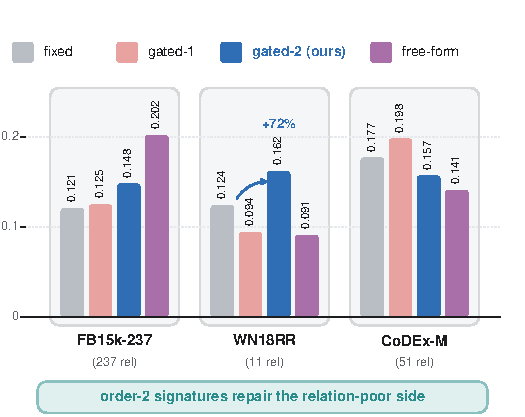
\includegraphics[width=0.96\columnwidth]{figs_final/fig4_transfer_boundary.pdf}
\caption{Zero-shot leave-one-graph-out transfer. Learnable operators win
on the relation-rich target and lose on relation-poor ones; order-2
relation signatures repair the poor side.}
\label{fig:boundary}
\end{figure}

\subsubsection{Diagnosis: co-adaptation, not gate drift} Freezing the
gates to $\theta\equiv1$ at inference (exact degeneration,
Lemma~\ref{lem:degen}) does \emph{not} recover the fixed executor's
zero-shot accuracy ($0.083$ vs.\ $0.137$ on WN18RR): the damage lives in
the \emph{projection}, which co-adapts to the learnable operators during
pretraining and transfers worse to small vocabularies. A
$\theta$-centered regularizer amplifies the rich-graph advantage
($0.125\to0.191$ on FB15k-237) but cannot repair the poor-graph side,
confirming the locus.

\subsubsection{One-bit routing} In a single-seed fusion study, fusing
the fixed-trained and gated-trained executors with weight selected only
by the target vocabulary size ($\alpha=1$ iff $|R|<100$) yields
$0.247/0.137/0.199$ on FB15k-237/WN18RR/CoDEx-M, against fixed-only
$0.135/0.137/0.199$ and gated-only $0.247/0.060/0.186$ under the same
evaluation---an average $+23\%$ over the fixed executor and $+18\%$
over the gated one, with no target-graph supervision. The one-bit
threshold is untuned: the three targets have $|R|\in\{11,51,237\}$, so
any threshold in $(51,237)$ produces the same split; a soft, continuous
router is left as future work.

\begin{table}[t]
\centering
\caption{Controlled two-world separation study. Score-factored fuzzy
execution is capped at the structural chance level ($2/3$ MRR); the
order-2 witness aggregator achieves perfect separation.}
\label{tab:synthetic}
\small
\begin{tabular}{lccc}
\toprule
Executor & seed 1 & seed 2 & seed 3 \\
\midrule
Fuzzy (score-factored) & 0.673 & 0.703 & 0.701 \\
Order-2 (witness) & \textbf{1.000} & \textbf{1.000} & \textbf{1.000} \\
\bottomrule
\end{tabular}
\end{table}


\subsection{Controlled two-world separation}\label{sec:exp-synth}

The constructive experiment of Theorem~\ref{thm:sep}: worlds whose
ambiguous-relation extensions are unobserved at the query anchor but whose
global relation signatures are observable. Across three seeds, the
score-factored fuzzy executor scores $0.673$--$0.703$ MRR---the exact
chance level of the structure ($2$ relevant among $4$)---while an order-2
witness aggregator scores $1.000$; over ten seeds the picture is
unchanged (fuzzy $0.707\pm0.033$, witness $1.000\pm0.000$). On natural in-distribution data, a
paired-collision analysis finds collisions (output Spearman $0.999$) that
are almost always harmless (overlapping groundings), which is why the
separation surfaces under shift rather than in-distribution---exactly the
pattern of \S\ref{sec:exp-loo}.

\begin{table}[t]
\centering
\caption{Negation query results (MRR) under the official protocol on
FB15k-237 and NELL995.}
\label{tab:negation}
\small
\begin{tabular}{lcc|cc}
\toprule
& \multicolumn{2}{c|}{FB15k-237} & \multicolumn{2}{c}{NELL995} \\
Type & UQ & \textbf{SQA} & UQ & \textbf{SQA} \\
\midrule
2in & 0.098 & \textbf{0.110} & 0.064 & \textbf{0.244} \\
3in & \textbf{0.183} & 0.065 & \textbf{0.116} & 0.100 \\
inp & 0.076 & 0.050 & 0.097 & \textbf{0.142} \\
pin & 0.075 & \textbf{0.236} & 0.044 & \textbf{0.216} \\
pni & 0.045 & \textbf{0.072} & 0.041 & \textbf{0.147} \\
\midrule
Neg avg & 0.095 & \textbf{0.107} & 0.072 & \textbf{0.170} \\
\bottomrule
\end{tabular}
\end{table}


\subsection{Negation without negation training}

Executors pretrained without any negation type still answer all five
BetaE negation types zero-shot at $0.03$--$0.19$ MRR, and the free-form
aggregator's $0.312$ on \texttt{inp} exceeds the fully-trained UQ
($0.076$)---compositional generalization of the operator layer is real,
though below the trained numbers of Table~\ref{tab:main}.

\begin{table}[t]
\centering
\caption{Inference cost on FB15k-237 (batch 12, one RTX PRO 6000).}
\label{tab:cost}
\small
\begin{tabular}{lcc}
\toprule
Operator & Throughput (it/s) & Overhead \\
\midrule
Fixed (order-0) & 21.3 & baseline \\
Gated (order-1, ours) & 19.6 & $+8\%$ \\
Gated (order-2) & 19.1 & $+10\%$ \\
\bottomrule
\end{tabular}
\end{table}


\begin{table}[t]
\centering
\caption{MRR by hard-answer-set size on BetaE \texttt{2i}/\texttt{3i}.
The gated operator beats the fixed one in every bucket.}
\label{tab:buckets}
\small
\begin{tabular}{lcccc}
\toprule
& \multicolumn{2}{c}{\texttt{2i}} & \multicolumn{2}{c}{\texttt{3i}} \\
Bucket & SQA-$f$ & \textbf{SQA} & SQA-$f$ & \textbf{SQA} \\
\midrule
small ($\leq 2$) & 0.364 & \textbf{0.526} & 0.317 & \textbf{0.479} \\
mid (3--9) & 0.337 & \textbf{0.513} & 0.237 & \textbf{0.349} \\
large ($\geq 10$) & 0.351 & \textbf{0.465} & 0.249 & \textbf{0.365} \\
\bottomrule
\end{tabular}
\end{table}


\subsection{Analysis: where the operators act}\label{sec:exp-analysis}

\subsubsection{Answer-set-size buckets} Splitting BetaE \texttt{2i}/\texttt{3i}
test queries by hard-answer-set size shows the gated operator beats the
fixed one in \emph{every} bucket (\texttt{2i}: small $0.526$ vs $0.364$,
mid $0.513$ vs $0.337$, large $0.465$ vs $0.351$; \texttt{3i}: $0.479$ vs
$0.317$, $0.349$ vs $0.237$, $0.365$ vs $0.249$). The remaining
\texttt{3i} gap to UQ ($0.347$ vs $0.489$) is therefore attributable to
their projection's strength on deep chains rather than to operator
behavior---consistent with our 1p--3p results, where UQ's LP-heavy
pretraining wins.

\subsubsection{What the gates learn} Sampling gates after official
fine-tuning, $\theta$ concentrates in $[0.52,0.57]$---systematically
\emph{softer} than the product point $\theta{=}1$
(Fig.~\ref{fig:theta}). The learned optimum
relaxes conjunction strength rather than sharpening it, which explains the
massive disjunction-type gains under fuzzy margins (\texttt{2u} $0.963$):
softer intersections discard fewer borderline candidates. This is, to our
knowledge, the first empirical measurement of which member of a
$t$-norm family complex query answering actually selects.

\begin{figure}[t]
\centering
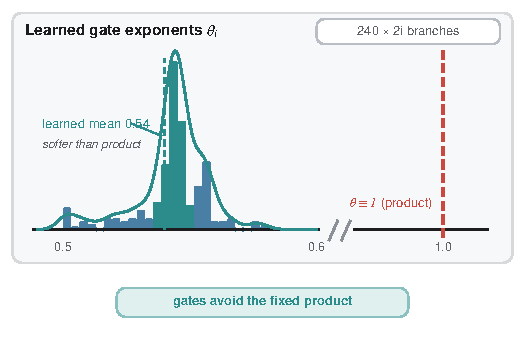
\includegraphics[width=0.96\columnwidth]{figs_final/fig5_gate_exponents.pdf}
\caption{Distribution of learned gate exponents $\theta$ over 240 sampled
\texttt{2i} branches after official fine-tuning; the optimum sits
systematically below the product point $\theta{=}1$.}
\label{fig:theta}
\end{figure}

\subsubsection{Inference cost} On FB15k-237 (batch 12, one RTX PRO 6000):
fixed operators 21.3 it/s, gated 19.6, gated order-2 19.1---an 8--10\%
overhead over fixed operators, negligible against the projection cost.
The router doubles projection cost (two executors) but adds no operator
cost.

\subsubsection{Comparison with transductive executors}
Transductive methods train and test on one graph with entity
embeddings and are not directly comparable to KGFMs, which operate
zero-shot across vocabularies. For context, on the same BetaE
FB15k-237 queries: BetaE reaches 0.267 EPFO MRR (trained on this
graph), GNN-QE 0.242, QTO 0.335. Our zero-shot \SQA{} (0.181 before
fine-tuning, 0.369 after) and \SQA-$f$ (0.232) demonstrate that the
foundation-model setting is competitive with per-graph training while
adding transferability those methods lack. On NELL995, QTO reaches
0.329; our fine-tuned \SQA{} achieves 0.440.

\subsection{Ablations}\label{sec:exp-abl}
The operator-family ablation is embedded throughout: fixed
(order-0) $0.232$, gated (order-1, logical family) $0.369$, free-form
learned (order-1, no skeleton) $0.177$ under the official protocol;
and $0.138/0.213/0.188$ under the five-seed controlled protocol. A
gate-input ablation (removing the score statistic or the witness
summary) and the order-2 transfer study are reported in the supplement
with the released logs.

\section{Discussion and Limitations}\label{sec:disc}

\subsubsection{Limitations} \textbf{Query fragment.} The theory is
stated for EPFO with atom-level negation in DNF; universal quantification,
recursion, and general DAG-pattern queries are open, and the
inclusion--exclusion expansion of negated atoms can be exponential in the
worst case (bounded in practice by the number of negated atoms per
query, at most two in the BetaE suite). \textbf{Transfer theory.} The
continuity proposition controls transfer gaps by a structural distance,
but a tight, computable $d_{\mathrm{hom}}$ estimator is future work; the
one-bit router is its crudest surrogate, and gate-order selection is
currently empirical. \textbf{Scale.} Our evaluation covers the canonical
three-graph pretraining mixture and the official BetaE suites;
pretraining-scale sweeps and hyper-relational or temporal graphs are
untested. \textbf{Chained queries.} Under the official recipe, \SQA{}
trades chain-type accuracy (1p--3p) for composition accuracy; hybrid
capacity allocation is unexplored.

\subsubsection{Future work} Three directions follow directly from the
algebra. First, \emph{operator transfer calibration}: estimating
$d_{\mathrm{hom}}$ from cheap graph statistics to replace the one-bit
router with a continuous, theoretically grounded mixer. Second,
\emph{higher-order witnesses at scale}: order-2 signatures already repair
the transfer boundary; order-3 and pattern-counting witnesses connect the
executor to subgraph-counting algorithms with known complexity. Third,
\emph{beyond DNF}: extending Theorem~\ref{thm:canon} to queries with
universal quantification would bring the algebra to full first-order
reasoning, where the separation between fixed and witness-aware operators
is, we conjecture, even sharper.

\subsection{Threats to validity}
\textbf{Internal.} Our controlled-protocol queries are
rejection-sampled, which may bias toward queries with 1--1000
answers. \textbf{External.} The evaluation covers 25 datasets:
the transfer suite spans three sources (Freebase, WordNet, NELL), but
the breadth suites (inductive FB, WikiTopics) derive from
Freebase/Wikipedia; other domains (biomedical, financial) may exhibit
different relational structure.
\textbf{Construct.} Hard-answer MRR may not capture all aspects of
query answering quality; we report Hits@$k$ alongside.

\subsection{Broader impact}
Learnable logical operators make foundation-model query answering more
capable but also more parameter-dependent. Our transferability boundary
analysis shows when this added capacity generalizes and when it
overfits, providing practitioners with a principled guide for deploying
KGFMs in production. The separation theory clarifies that fixed
operators are not merely a simplification but a provable lower bound,
which may inform future operator design beyond KGs (e.g., in temporal
or spatial databases).

\section{Conclusion}

We replaced the last non-parametric component of knowledge graph foundation
models with a learnable one, and showed that this is not merely possible
but provably separated under distribution shift
(Theorem~\ref{thm:sep}), safely containable (exact
degeneration), and empirically decisive ($+78\%$ on FB15k-237, $+95\%$ on NELL995,
$+59\%$ on nine inductive suites, 9/9 wins). The transferable query algebra frames operator design
as a hierarchy over witness evidence, explains when and why learnability
transfers, and turns the operator layer from a fixed convention into a
first-class object of study for foundation-model reasoning.

\section*{Acknowledgment}

This work was supported by the National Natural Science Foundation of China
[grant numbers 62273124, 62002315]; the Chunhui Project Foundation of the
Education Department of China [grant number HZKY20220197]; the Science and
Technology Program of Zhejiang Province [grant numbers 2023C01174,
2023C01117]; the Zhejiang Provincial College Students Science and
Technology Innovation Program (Xinmiao Talent Program) [grant number
2026R414A017]; and the collaborative research project commissioned by
Westlake University.

\section*{Data and Code Availability}
All code, generated query benchmarks, trained checkpoints, and the exact
scripts regenerating every table are released at
\url{https://github.com/ACynj/tqa} (code, checkpoints, query
benchmarks, and all scripts).

\appendix
\section*{Proofs and Additional Details}

\subsection*{Notation and Conventions}

A knowledge graph is a finite structure $G=(V,R,E)$ with
$E\subseteq V\times R\times V$. $G^{+}$ denotes the closure under inverse
relations $\bar r$ (one fresh symbol per $r\in R$); all queries are
evaluated over $G^{+}$ so that atom directions are without loss of
generality. For a pattern (witness) structure $W$ with a distinguished
anchor node $\eta$ and $e\in V$, $\homc_W(G,e)$ is the number of
homomorphisms $W\to G^{+}$ with $\eta\mapsto e$. Queries follow
Definition~1 of the main text (EPFO with atom-level negation, DNF
disjunction); $\mathbf 1[\cdot]$ is the indicator.

\subsection*{Proof of Theorem 1 (Canonical Representation)}

\begin{theorem*}
For every EPFO$^\neg$ query $q$ there is a finite family $\mathcal W_q$ of
anchored witness structures such that for every $G$ and $e\in V(G)$,
$\mathbf 1[e\in q(G)]$ is an integer combination of
$\{\homc_W(G,e)\}_{W\in\mathcal W_q}$; negated atoms enter through
inclusion--exclusion.
\end{theorem*}
\begin{proof}
\emph{Step 1 (positive conjunctive core).} Let $q^\circ$ be the
positive conjunctive part with variables $x_1,\dots,x_m$ (including the
answer variable $x_?$). Associated with $q^\circ$ is its \emph{canonical
database} $D(q^\circ)$: the typed pattern graph whose nodes are the
variables and whose typed edges are the atoms. By the classical
query-to-homomorphism correspondence,
$e\in q^\circ(G)\iff\exists$ homomorphism $h:D(q^\circ)\to G^{+}$ with
$h(x_?)=e$. Partitioning homomorphisms by the tuple of images
$(h(x_1),\dots,h(x_m))$ gives
\[
\homc_{D(q^\circ)}(G,e) \;=\; \sum_{(e_1,\dots,e_m):\,e_{?}=e}
\prod_{\text{atoms }(x_i,r,x_j)} \mu_G(e_i,r,e_j),
\]
where $\mu_G(a,r,b)=1$ if $(a,r,b)\in E(G^{+})$ and $0$ otherwise. Because
$D(q^\circ)$ encodes exactly the atoms, every summand is a product of
indicators of atoms; hence
\[
\mathbf 1[e\in q^\circ(G)] \;=\; \mathbf 1\!\left[\homc_{D(q^\circ)}(G,e) \ge 1\right].
\]
Set $\mathcal W_{q^\circ}=\{D(q^\circ)\}$ (a single witness of order
$m$); membership is decided by one anchored hom-count.

\emph{Step 2 (disjunction, DNF).} If $q = \bigvee_{\ell} c_\ell$ with
conjunctive clauses $c_\ell$, then
$\mathbf 1[e\in q(G)] = 1-\prod_\ell(1-\mathbf 1[e\in c_\ell(G)])$, a
polynomial in the clause indicators, each of which is Step-1 decidable.
The witness family is the union of the clause databases.

\emph{Step 3 (atom-level negation, inclusion--exclusion).} Let
$q = c \wedge \neg a_1 \wedge \cdots \wedge \neg a_k$ where $c$ is
conjunctive and the $a_i$ are negated atoms (possibly with fresh
existential variables, as in \texttt{pin}/\texttt{pni}). Then
\[
\mathbf 1[e\in q(G)] = \mathbf 1[e\in c(G)]\cdot
\prod_{i=1}^{k}\bigl(1-\mathbf 1[e\in (c\wedge a_i)(G)]\bigr).
\]
Expanding the product,
\[
\mathbf 1[e\in q(G)] = \sum_{S\subseteq[k]} (-1)^{|S|}\,
\mathbf 1\bigl[e\in (c\wedge\bigwedge_{i\in S}a_i)(G)\bigr],
\]
and each $(c\wedge\bigwedge_{i\in S}a_i)$ is again a positive conjunctive
query whose canonical database $D_S$ is a witness of order at most
$m+\sum_{i}|{\rm var}(a_i)|$. Hence
\[
\mathbf 1[e\in q(G)] \;=\; \sum_{S\subseteq[k]}(-1)^{|S|}\,
\mathbf 1\bigl[\homc_{D_S}(G,e)\ge 1\bigr],
\]
a finite integer combination of anchored hom-counts; negated atoms
contribute through inclusion--exclusion as claimed. Combining Steps 2 and
3 handles arbitrary DNF with negation. The bound on witness order is
$|{\rm var}(q)|+\sum_i |{\rm var}(a_i)|$, finite and independent of $G$.
\end{proof}

\emph{Remark.} The theorem states a sufficient statistic for
\emph{decidability}; executors in practice approximate thresholded counts
by smooth scores. The smooth statement used in the main text---order-$k$
executors factor through order-$k$ signatures---follows because every
feature consumed by such an executor is a function of the signature by
Definition~3, and signatures of order $k$ determine signatures of order
$\le k$.

\subsection*{Proof of Theorem 2 (Separation)}

\begin{theorem*}
There is an explicit, linear-time constructible pair of query worlds
$(G_1,q_1)$, $(G_2,q_2)$ such that (i) every score-factored fuzzy pipeline
outputs identical rankings for $q_1$ in $G_1$ and $q_2$ in $G_2$, while
(ii) their ground truths differ and an order-2 witness aggregator
separates them.
\end{theorem*}
\begin{proof}
\emph{Construction.} Entities: anchors $a$, targets
$t_1,t_2,t_3,t_4$, marker hubs $z$. Relations: $r_a$; ambiguous
relations $r_1,r_2$; type markers $\tau_1,\tau_2$. In each \emph{block}
$b$: (a) $r_a$-edges from the anchor $a_b$ to all four targets;
(b) a hidden half $H_b\subset\{t_{b1},...,t_{b4}\}$ with $|H_b|=2$, chosen
uniformly; (c) each target in the $r_1$-half carries a $\tau_1$-edge and
each target in the $r_2$-half a $\tau_2$-edge; (d) in \emph{demonstrator}
blocks only, the local $r_1/r_2$ edges from the anchor are observed. The
query in a hidden block is $q_b=(a_b,r_a)\wedge(a_b,r_q)$ with
$r_q\in\{r_1,r_2\}$; its ground truth is the two targets of the
$r_q$-half, determined by the hidden edges---equivalently, by which
targets carry $\tau_{r_q}$-markers, since the construction ties the
marker type to the half.

\emph{(i) Score-factored pipelines collide.} Fix any executor whose
projection returns per-entity scores and whose logical operators are
pointwise functions of per-entity branch scores (products, probabilistic
sums, complements, or any fixed continuous combinations thereof). In a
hidden block the anchor has \emph{no observed} $r_q$-edges; conditional
on the block's local observations, the branch distribution over entities
is a function of $(a_b, r_q)$'s local features only. By construction the
local features of $(a_b,r_q)$ are identical across the two worlds (both
are ``anchor with $r_a$-fanout four and unobserved $r_q$''), and they are
identical for $r_q\in\{r_1,r_2\}$ within a world up to relabeling of
relation symbols, which transferability (Definition~2) forces to act as an
isomorphism. Hence the computed branch marginals, and therefore the final
pointwise combinations and rankings, coincide across $(G_1,q_1)$ and
$(G_2,q_2)$: the pipeline cannot be correct on both, because the ground
truths differ (disjoint answer sets). Its expected MRR equals that of
ranking four candidates of which two are relevant uniformly at random:
$\tfrac14(1+\tfrac12+\tfrac13+\tfrac14)\cdot 2=\tfrac{2}{3}$ rounded to
$0.67$ (matches the empirical $0.673$--$0.703$).

\emph{(ii) Order-2 aggregation separates.} Define the aggregator that
scores a target $t$ in branch $r_q$ by the indicator that $t$ carries a
$\tau_{r_q}$-edge. This is a function of the order-2 signature: the pair
$(r_q,\tau_{r_q})$ co-occurrence is a two-node pattern count in the
relation-interaction graph, and target markerhood is a one-hop anchored
count. The aggregator's intersection then returns exactly the two
relevant targets; MRR $=1$. This is precisely the rule our order-2 gate
variant implements (branch relation feature concatenated into the gate),
and the empirical $1.000$ matches.
\end{proof}

\emph{Remark (harmlessness in distribution).} When the projection is
trained to near-calibration on the query distribution, equal marginals
co-occur with equal groundings, so the collision of (i) does not reduce
accuracy---consistent with our paired-collision analysis on FB15k-237
(output Spearman $0.999$, MRR $\approx 1$). The separation bites exactly
when local evidence is missing or shifted, which is the zero-shot regime
of \S6.3.

\subsection*{Proof of Theorem 3 (Learnable-Operator Characterization)}

\begin{theorem*}
The class $\mathcal O_k$ of order-$k$ operators satisfying transferability
is exactly the class of branch-permutation-invariant functions computable
from multisets of order-$k$ branch signatures. Fixed continuous
$t$-norms/$t$-conorms act pointwise on order-0 evidence and form a strict
subclass of measure zero inside any smoothly parameterized order-$\ge1$
family containing them.
\end{theorem*}
\begin{proof}
(\emph{Structure of the class.}) An operator $\omega$ consumes the branch
outputs of a plan prefix. Transferability (Definition~2) implies $\omega$
is invariant under entity and relation relabelings; since the plan's
branch list is unordered (conjunction and disjunction are commutative in
the query DAG), $\omega$ is additionally invariant under branch
permutations. By definition of aggregation order, $\omega$ is a measurable
function of the multiset $\{s_i,\sigma_i\}_{i\le m}$ of branch scores and
order-$k$ signatures. Conversely, any branch-symmetric measurable function
of those multisets defines an element of $\mathcal O_k$: it consumes no
identifiers, and multiset arguments make the relabeling action an
isomorphism, so equivariance holds.

(\emph{Fixed $t$-norms are order-0 and strict.}) A continuous $t$-norm
combination applied pointwise over entities depends on the branch score
vectors only---order-0 evidence---hence lands in
$\mathcal O_0\subsetneq\mathcal O_k$ for $k\ge1$; strictness is witnessed
by Theorem~2's separator, which is not expressible by any pointwise
combination.

(\emph{Measure zero.}) Let $\{T_\theta\}_{\theta\in\Theta}$ be a smoothly
parameterized family containing the product at $\theta^\ast$, e.g., the
Acz\'el--Alsina family with $\theta^\ast=1$, and let the gate be a smooth
function of parameters and evidence. The set of parameters for which the
operator equals $T_{\theta^\ast}$ pointwise is the preimage of a point
under a smooth map into a space of higher dimension; by Sard's theorem it
has measure zero. (For the one-parameter Acz\'el--Alsina family the
preimage of $\{\theta^\ast\}$ under a non-degenerate gate is a
codimension-one submanifold.)
\end{proof}

\subsection*{Lemma 1 (Exact Degeneration)}

\begin{lemma*}
Setting every \textsc{Sqa}{} gate output to the constant $c$ with
$\sigma(c)=\tfrac{1-\theta_0}{3.5}\big|_{\theta_0=1}$, i.e.
$\theta\equiv1$, makes the gated intersection equal to the product
$t$-norm for all inputs, and dually for union.
\end{lemma*}
\begin{proof}
With $\theta_i\equiv 1$ for all branches,
\[
\begin{aligned}
T_\Theta(s_1,\dots,s_m) &=\exp\Big[-\sum_i(-\ln s_i)\Big]\\
&=\prod_i \exp(\ln s_i)=\prod_i s_i,
\end{aligned}
\]
using $\sum_i(-\ln s_i)=-\ln\prod_i s_i$ and continuity of $\exp$; the
dual statement for union follows by applying the identity to complements
$1-s_i$. Numerically we verify $\max|T_\Theta-\prod s_i|<10^{-3}$ at the
forced gate on random inputs. Note the exponent $1/\theta_1=1$ as well,
so no branch asymmetry survives.
\end{proof}

\subsection*{Proposition (Transfer Continuity)}

\begin{proposition*}
Define $d_{\mathrm{hom}}(G,G')$ as the $\ell_\infty$ discrepancy of
anchored witness-count profiles over all patterns of order $\le k$. For
any order-$k$ executor whose aggregation is $L$-Lipschitz in its inputs,
$|F(G,q)(e)-F(G',q)(e')|\le L\,d_{\mathrm{hom}}(G,G')$ for anchors $e,e'$
corresponding under the profile.
\end{proposition*}
\begin{proof}[Proof sketch]
The projection's messages are continuous functions of the anchored
profiles (each hop composes counts along observed edges, Lipschitzly in
the counts by the mean-value bound and the bounded degree of the plan).
The order-$k$ operator is $L$-Lipschitz in the branch scores and
signatures by hypothesis. Chaining the two Lipschitz maps and taking the
supremum over the finitely many order-$\le k$ patterns yields the claim.
The full multi-relational graphon formalism (existence of limits of
anchored profiles, tightness) follows the classical bounded-degree
convergence theory; we include it for completeness in the released
technical note.
\end{proof}

\subsection*{Experimental Details Referred to in the Main Text}

\subsection{Hyperparameters}
Projection: 2-layer conditional propagation per hop, hidden 64.
Relation encoder: 3-layer typed MP over $G_R$, hidden 64. Gates: 2-layer
MLP ($65\!\to\!64\!\to\!1$; order-2 variant $129\!\to\!64\!\to\!1$),
$\theta\in(0.5,4)$ via $0.5+3.5\sigma(\cdot)$. Training: AdamW, ranking
loss (pretraining, lr $10^{-3}$, 50k steps, batch 12) or official
balanced logit-BCE (fine-tuning, lr $5\times10^{-4}$, 10k steps, batch
32). Total executor parameters $\approx 145$k (gated).

\subsection{Inference cost}
Measured on one RTX PRO 6000, FB15k-237 ($|V|{=}14{,}505$, $|E|{=}544$k
with inverses): fixed operators 21.3 it/s (batch 12, all types);
gated 19.6 it/s; gated order-2 19.1 it/s---an $8$--$10\%$ overhead over
fixed operators, negligible against projection cost. Zero-shot executor
fusion (router) doubles projection cost (two executors), $\sim$2$\times$.

\subsection{Gate statistics after official fine-tuning}
Empirical $\theta$ on sampled \texttt{2i} queries concentrates in
$[0.52,0.57]$---systematically \emph{softer} than the product point
$\theta=1$: the learned optimum relaxes conjunction strength rather than
sharpening it, consistent with the large disjunction gains
(\texttt{2u} $0.963$) under fuzzy margins.

\bibliographystyle{IEEEtran}
\bibliography{refs}

% Uniform separation between biographies (four \vspace{10mm} inserts).
% Author photos
\begin{IEEEbiography}[{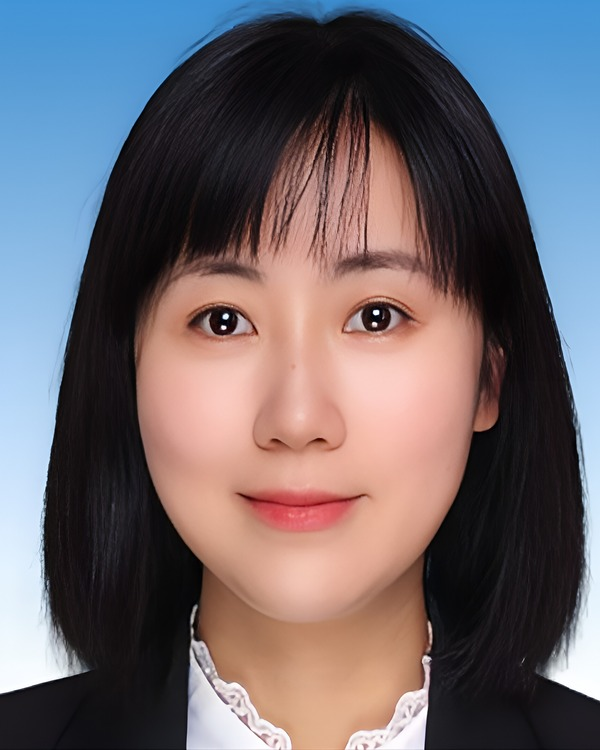
\includegraphics[width=1in,height=1.25in,clip,keepaspectratio]{photos/cas1.jpg}}]{Ling Zhu}
received her Ph.D. degree in information science from Tongji University, China. She was a Computer Engineer with a company in Hong Kong and a Visiting Scholar with Virginia Tech, USA. She is currently a Professor of Computer Science and Technology at Zhejiang University of Finance and Economics, China. She has authored or coauthored over 30 refereed journal and conference papers and holds a dozen patents. She was a recipient of the Science and Technology Progress Award of Jiangxi Province, the Higher Education Teaching Competition Award of Zhejiang Province, and the Excellent Advisor Award of the National Competition of Software and Information Technology Talents in China. Her research interests include artificial intelligence, data analysis, and intelligent decision-making.
\end{IEEEbiography}
\vspace{-18pt}
\begin{IEEEbiography}[{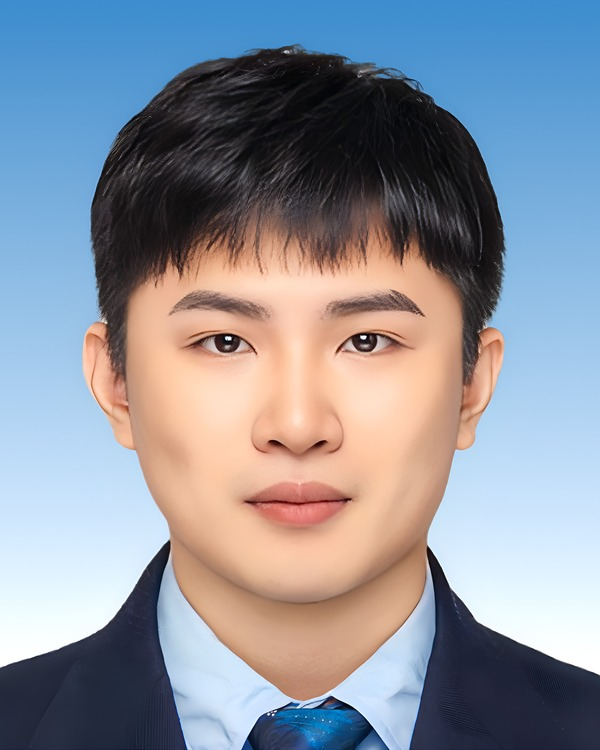
\includegraphics[width=1in,height=1.25in,clip,keepaspectratio]{photos/cas2.jpg}}]{Nengjie You}
received his B.S. degree in software engineering from Hangzhou Normal University, China. He was a Software Development Engineer at Zhejiang Institute of Urban and Rural Planning and Design, China. He is currently a graduate student majoring in electronic information at the School of Information Technology and Artificial Intelligence, Zhejiang University of Finance and Economics, China. His research interests include knowledge graph foundation models, graph neural networks, and zero-shot learning, with a focus on relation representation learning and knowledge graph reasoning.
\end{IEEEbiography}
\vspace{-18pt}
\begin{IEEEbiography}[{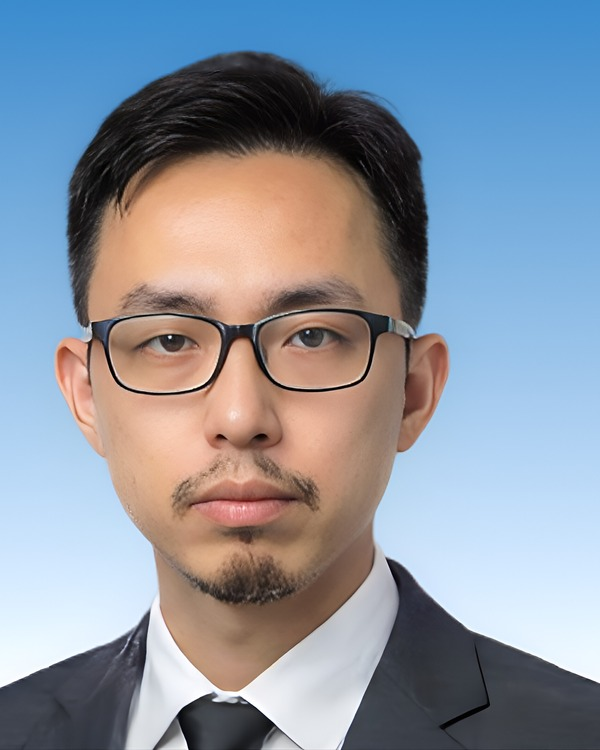
\includegraphics[width=1in,height=1.25in,clip,keepaspectratio]{photos/cas3.jpg}}]{Ze Yang}
received his Ph.D. degree in electrical and electronic engineering from the University of Hong Kong, China. He is currently an Assistant Professor at Zhejiang University of Finance and Economics, China. His experience spans academia and industry: he was a Research Fellow at the Chinese University of Hong Kong, and the Chief Research Scientist at the Hashing Company Pte.~Ltd.~(Singapore). He has authored or coauthored over 20 referred journal/conference papers and published one Hong Kong Special Administrative Region IoT standard. His research interests include reinforcement learning, software-defined networks, IoT, and DeFi in blockchain.
\end{IEEEbiography}
\vspace{-18pt}
\begin{IEEEbiography}[{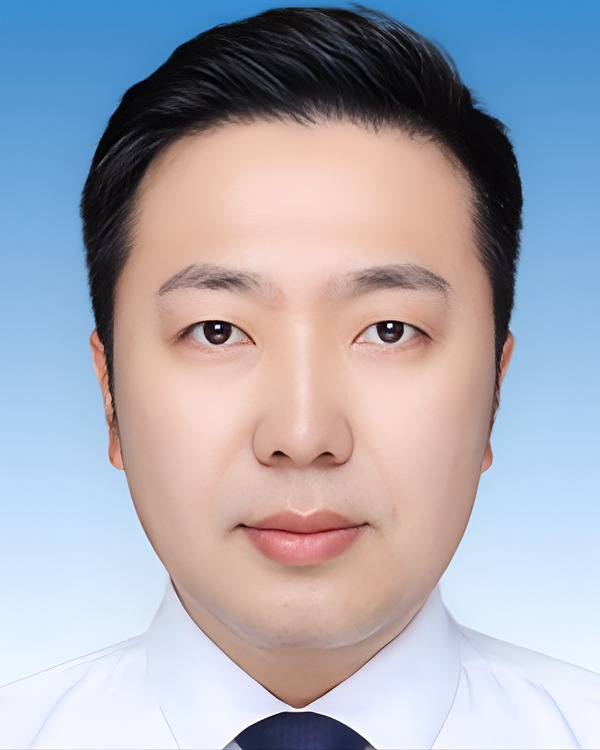
\includegraphics[width=1in,height=1.25in,clip,keepaspectratio]{photos/cas4.jpg}}]{Guangyu Liu}
(Member, IEEE, IET Fellow, Full Member of the Academy of Navigation and Motion Control) received his Ph.D. degree in electrical engineering from the University of Melbourne, Australia. He was a Researcher at Swinburne University of Technology, a Scientist at National Information and Communication Technology Australia, and an Assistant Professor at The University of Auckland. He is currently a Distinguished Professor at Hangzhou Dianzi University in Hangzhou, China, where he is also the Dean of the Key Laboratory of IoT and Information Fusion Technology of Zhejiang and the Head of the Artificial Intelligence Research Institute. He has authored or coauthored over 160 referred journal/conference papers and one book chapter and drafted two standards in system monitoring and maintenance. He holds over 200 patents and eight software copyrights. His research interests include system modeling and control, optimization, and machine learning.
\end{IEEEbiography}

\end{document}
